\begin{enumerate}[label=\thesubsection.\arabic*,ref=\thesubsection.\theenumi]


\item Find the values of $k$ for which the line 
\begin{align}
(k-3)x-(4-k^2)y+k^2-7k+6=0 \label{eq:chapters/11/10/4/1/1}
\end{align}
is
\begin{enumerate}
\item Parallel to the $x$-axis
\item Parallel to the $y$-axis
\item Passing through the origin
\end{enumerate}
    \solution 
		The parameters of the given line are
\begin{align}
\vec{n}^{\top}\vec{x}=c \label{eq:chapters/11/10/4/1/2}
\end{align}
This equation can be expressed in the form of 
\begin{align}
\vec{n} = \myvec{k-3\\-4+k^2}, c  = -k^2+7k-6
\end{align}
\iffalse
Then \eqref{eq:chapters/11/10/4/1/1} can be expressed as
\begin{align}
\myvec{k-3 & -4+k^2}\vec{x} &=-k^2+7k-6\label{eq:chapters/11/10/4/1/4}
\end{align}
\fi
\begin{enumerate}
%part-1
    \item 
	    In this case,
	    \iffalse
The normal vector of $x$-axis is given by
\begin{align}
\myvec{0\\1}
\end{align}
\fi
equating $\vec{n}$ to the normal vector of $x$-axis,
\begin{align}
\myvec{k-3\\-4+k^2} &=\alpha\myvec{0\\1}\label{eq:chapters/11/10/4/1/6}
\\
\implies
k &=3
\end{align}
Substituting the value of $k$ in \eqref{eq:chapters/11/10/4/1/1}, the desired equation is
\begin{align}
        \myvec{0 & 5}\vec{x} &=6
\end{align}

\item In this case, 
equating $\vec{n}$ to the normal vector of $y$-axis,
\begin{align}
\myvec{k-3\\-4+k^2} &=\beta\myvec{1\\0}\label{eq:chapters/11/10/4/1/11}
\\
	\implies k &=\pm2
\end{align}
Substituting the value of $k$ in \eqref{eq:chapters/11/10/4/1/1}, the desired equation is 
\begin{align}
        \myvec{-1 & 0}\vec{x} &=4, \quad  k &=2\\
        \myvec{-5 & 0}\vec{x} &=-24, \quad  k &=-2
\end{align}
\item 
	In this case, 
\begin{align}
	c = 0 \implies 
	-k^2+7k-6 &= 0\\
	\implies k =1 \text{ or } k&=6
\end{align}
Substituting the value of $k$ in \eqref{eq:chapters/11/10/4/1/1}, the desired equations are 
\begin{align}
        \myvec{-2 & -3}\vec{x} &=0, \quad  k &=1\\
       \myvec{3 & 32}\vec{x} &=0, \quad  k &=6
\end{align}
\end{enumerate}

	\item Find the values of $\theta \text{ and } p$, if the equation $x\cos\theta+y\sin\theta=p$ is the normal form
of the line $\sqrt{3}x+y+2=0$.
\\
\solution
				\begin{align}
	\vec{n}=\myvec{\sqrt{3}\\1},
			c=-2
			\\
			\implies
			\theta=\tan^{-1}\brak{\sqrt{3}}
			=\frac{\pi}{3},
			p=\frac{\abs{c}}{\norm{\vec{n}}}=1
		\end{align}
See \figref{fig:chapters/11/10/4/2/Fig1}.
\begin{figure}[H]
	\begin{center} 
	    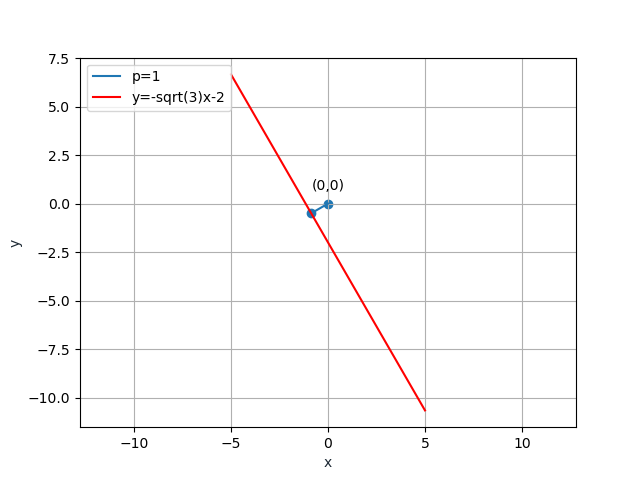
\includegraphics[width=0.75\columnwidth]{chapters/11/10/4/2/figs/line.png}
	\end{center}
\caption{}
\label{fig:chapters/11/10/4/2/Fig1}
\end{figure}


	\item Find the  equations of the lines, which cutoff intercepts on the axes  whose sum and product are 1 and -6 respectively.
\\
\solution
		Let the intercepts be $a$ and  $b$. Then
\begin{align}
a+b=1,
ab=-6 \label{eq:11/10/4/32a}
\\
\implies  a = 3, b = -2
\end{align}
Thus, the possible 
intercepts are
\begin{align}
\myvec{3\\0}, \myvec{0\\-2},
\myvec{-2\\0}, \myvec{0\\3}
\end{align}
From
		\eqref{prop:lin-eq-unit-mat},
\begin{align}
	\myvec{3 & 0 \\ 0 &-2}\vec{n} = \myvec{1 \\ 1}
	\\
	\implies \vec{n} = \myvec{\frac{1}{3} \\ -\frac{1}{2}}
	\\
	\text{or, } \myvec{2 & -3}\vec{x} = 6
\end{align}
using		\eqref{prop:lin-eq-unit}.
Similarly, the other line can be obtained
as
\begin{align}
	\myvec { 3 & -2 }  \vec{x}  = -6        
\end{align}
See  
\figref{fig:11/10/4/3line segmenta}.
\begin{figure}[!htbp]
\centering
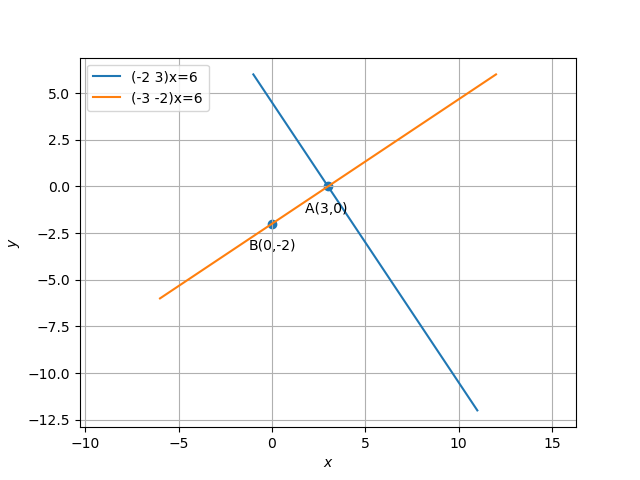
\includegraphics[width=\columnwidth]{chapters/11/10/4/3/figs/inter.png}
\caption{}
\label{fig:11/10/4/3line segmenta}
\end{figure}

	\item  Find the equation of the line parallel to y-axis and drawn through the point of
intersection of the lines x – 7y + 5 = 0 and 3x + y = 0.
\\
\solution
		\iffalse
\documentclass[12pt]{article}
\usepackage{graphicx}
\usepackage{amsmath}
\usepackage{mathtools}
\usepackage{gensymb}
\usepackage[utf8]{inputenc}
\usepackage{float}
\newcommand{\mydet}[1]{\ensuremath{\begin{vmatrix}#1\end{vmatrix}}}
\providecommand{\brak}[1]{\ensuremath{\left(#1\right)}}
\providecommand{\norm}[1]{\left\lVert#1\right\rVert}
\newcommand{\solution}{\noindent \textbf{Solution: }}
\newcommand{\myvec}[1]{\ensuremath{\begin{pmatrix}#1\end{pmatrix}}}
\let\vec\mathbf

\begin{document}
\begin{center}
\textbf\large{CLASS-11 \\ CHAPTER-10 \\ STRAIGHT LINES}
\end{center}
\section*{Excercise 10.4}

\section*{Solution}
\fi
The given line can be expressed as
\begin{align}
\myvec{1&-7}\vec{x}&=-5\\
\myvec{3&1}\vec{x}&=0
\end{align}
The intersection of two lines is given by row reducing the augmented matrix
\begin{align}
\myvec{
1&-7&5\\
3&1&0
}
\xleftrightarrow[]{R_2=R_2-3R_1}
\myvec{
1&-7&5\\
0&22&-15
}\\\xleftrightarrow[]{R_2=\frac{R_2}{22}}
\myvec{
  1&-7&5\\[1pt]
0&1&-\frac{15}{22}
}
\xleftrightarrow[]{R_1={R_1}+7{R_2}}
\myvec{
1&0&\frac{5}{22}\\[1pt]
0&1&\frac{-15}{22}
}
\end{align}
yielding
\begin{align}
  \vec{P}&=\myvec{-\frac{5}{22}\\[1pt] \frac{15}{22}}
\end{align}
The normal vector of the desired 
line is 
\begin{equation}
    \vec{n}=\myvec{1\\0}
    \label{eq:chapters/11/10/4/6/normal}
\end{equation}
The desired equation is then given by 
\begin{align}
	\vec{n}^{\top}\myvec{\vec{x}-\vec{P}}&=0
	\\
\implies 
	\myvec{1&0}\vec{x}&=-\frac{5}{22}
\end{align}
See Fig. 
\ref{fig:chapters/11/10/4/6/Fig3}
\begin{figure}[!ht]
  \begin{center} 
      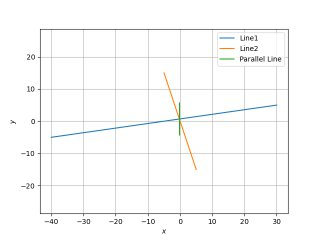
\includegraphics[width=\columnwidth]{chapters/11/10/4/6/figs/line_fig.png}
  \end{center}
\caption{}
\label{fig:chapters/11/10/4/6/Fig3}
\end{figure}

	\item Find the area of triangle formed by the lines $y-x=0, x+y=0, \text{ and } x-k=0$.
		\\
\solution
		The vertices of the triangle can be expressed using the equations
\begin{align}
	\myvec{1&1\\-1&1} \vec{A} &= \vec{0}
	\\
	\myvec{1&1\\1&0} \vec{B} &= \myvec{0\\k}
	\\
	\myvec{1&0\\-1&1} \vec{C} &= \myvec{k\\0}
\end{align}
from which
\begin{align}
\vec{A} = \myvec{0\\0},
	\vec{B}=\myvec{k\\-k},
	\vec{C}=\myvec{k\\k}
\end{align}
are trivially obtained.
Thus, 
\begin{align}
ar(ABC) &=\frac{1}{2}\norm{(\vec{A}-\vec{B})\times(\vec{A}-\vec{C})}\\
	&=\frac{1}{2}\norm{\myvec{-k\\k}\times\myvec{-k\\-k}}
=k^2
\end{align}

\item A ray of light passing through the point $\brak{1, 2}$ reflects on the x-axis at point $\vec{A}$ and the reflected ray passes through the point $\brak{5, 3}$. Find the coordinates of $\vec{A}$.
\\
    \solution 
		%	From \eqref{eq:11/10/4/22},
the reflection of $\vec{Q}$ is 
\begin{align}
\vec{R}  
= \myvec{5\\-3}
\end{align}
Letting
\begin{align}
\vec{A} = \myvec{x\\0},
\end{align}
since 
$\vec{P},
\vec{A},  
\vec{R}  
$
are collinear, 
		from \eqref{prop:lin-dep-rank},
\begin{align}
	\myvec{
		1 & 1 & 2 
		\\ 
		1 & 5 & -3 
		\\
		1 & x & 0 }
	\xleftrightarrow[R_3=R_3 - R_1]{R_2 = R_2 - R_1}
	\myvec{
		1 & 1 & 2 
		\\ 
		0 & 4 & -5 
		\\
		0 & x-1 & -2 }
	\\
	\xleftrightarrow[]{R_3 = 4R_3 - \brak{x-1}R_2}
	\myvec{
		1 & 1 & 2 
		\\ 
		0 & 4 & -5 
		\\
		0 & 0 & 5x-13 }
	\implies x = \frac{13}{5}
\end{align}
See  
\figref{fig:chapters/11/10/4/22/1}.
\begin{figure}[H]
\centering
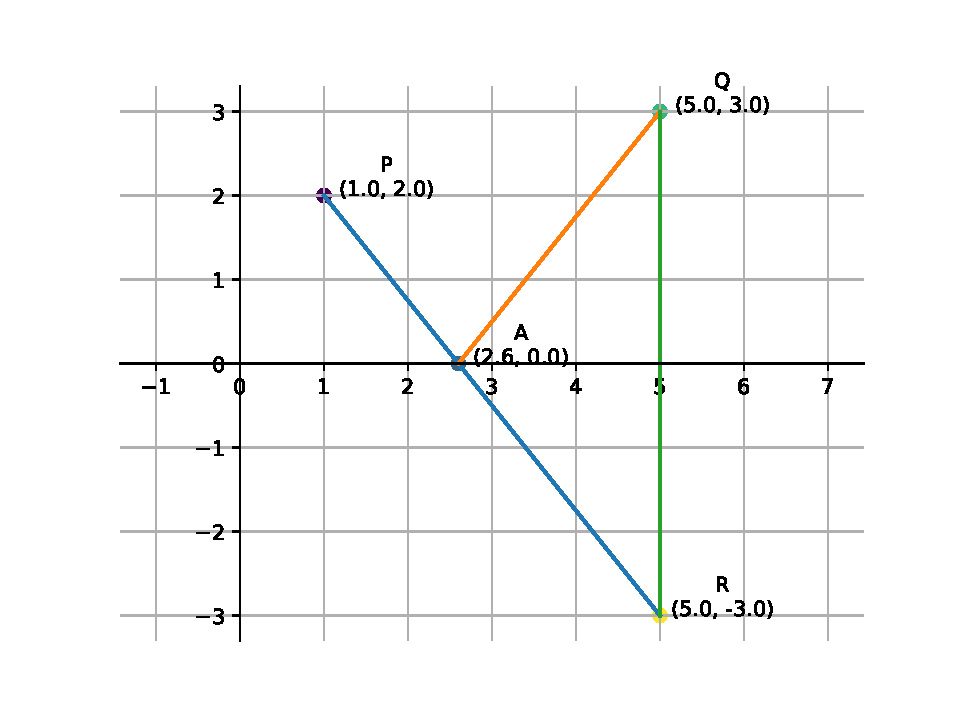
\includegraphics[width=0.75\columnwidth]{chapters/11/10/4/22/figs/fig.pdf}
\caption{}
\label{fig:chapters/11/10/4/22/1}
\end{figure}




%\item Find the equations of the lines, which cut-off intercepts on the axes whose sum and product are 1 and -6, resspectively.
%	\\
%    \solution 
%		%Let the intercepts be $a$ and  $b$. Then
\begin{align}
a+b=1,
ab=-6 \label{eq:11/10/4/32a}
\\
\implies  a = 3, b = -2
\end{align}
Thus, the possible 
intercepts are
\begin{align}
\myvec{3\\0}, \myvec{0\\-2},
\myvec{-2\\0}, \myvec{0\\3}
\end{align}
From
		\eqref{prop:lin-eq-unit-mat},
\begin{align}
	\myvec{3 & 0 \\ 0 &-2}\vec{n} = \myvec{1 \\ 1}
	\\
	\implies \vec{n} = \myvec{\frac{1}{3} \\ -\frac{1}{2}}
	\\
	\text{or, } \myvec{2 & -3}\vec{x} = 6
\end{align}
using		\eqref{prop:lin-eq-unit}.
Similarly, the other line can be obtained
as
\begin{align}
	\myvec { 3 & -2 }  \vec{x}  = -6        
\end{align}
See  
\figref{fig:11/10/4/3line segmenta}.
\begin{figure}[!htbp]
\centering
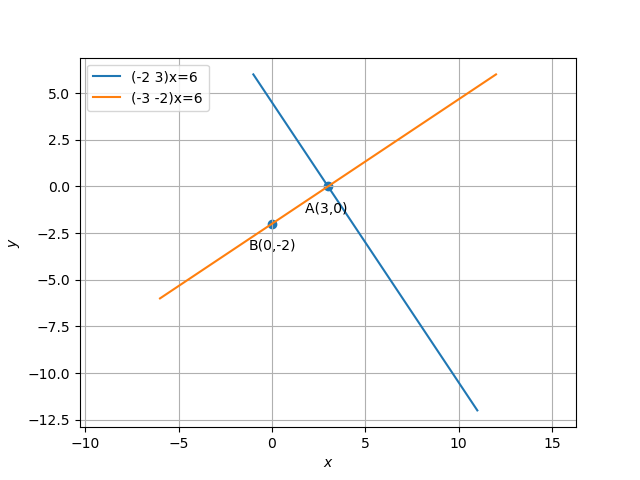
\includegraphics[width=\columnwidth]{chapters/11/10/4/3/figs/inter.png}
\caption{}
\label{fig:11/10/4/3line segmenta}
\end{figure}

    \item A person standing at the junction (crossing) of two straight paths 
    represented by the equations 
    \begin{align}
        \myvec{2&-3}\vec{x} = -4 
        \label{eq:chapters/11/10/4/24/L1}
    \end{align}
    and
    \begin{align}
        \myvec{3&4}\vec{x} = 5
        \label{eq:chapters/11/10/4/24/L2}
    \end{align} 
    wants to reach the path whose equation is 
    \begin{align}
        \myvec{6&-7}\vec{x} = -8
        \label{eq:chapters/11/10/4/24/L3}
    \end{align}
    Find equation of the path that he should follow.
\\
    \solution 
		%\iffalse
\documentclass[journal,12pt,twocolumn]{IEEEtran}
\usepackage{setspace}
\usepackage{gensymb}
\usepackage{xcolor}
\usepackage{caption}
\singlespacing
\usepackage{siunitx}
\usepackage[cmex10]{amsmath}
\usepackage{mathtools}
\usepackage{hyperref}
\usepackage{amsthm}
\usepackage{mathrsfs}
\usepackage{txfonts}
\usepackage{stfloats}
\usepackage{cite}
\usepackage{cases}
\usepackage{subfig}
\usepackage{longtable}
\usepackage{multirow}
\usepackage{enumitem}
\usepackage{mathtools}
\usepackage{listings}
\usepackage{tikz}
\usetikzlibrary{shapes,arrows,positioning}
\usepackage{circuitikz}
\let\vec\mathbf
\DeclareMathOperator*{\Res}{Res}
\renewcommand\thesection{\arabic{section}}
\renewcommand\thesubsection{\thesection.\arabic{subsection}}
\renewcommand\thesubsubsection{\thesubsection.\arabic{subsubsection}}

\renewcommand\thesectiondis{\arabic{section}}
\renewcommand\thesubsectiondis{\thesectiondis.\arabic{subsection}}
\renewcommand\thesubsubsectiondis{\thesubsectiondis.\arabic{subsubsection}}
\hyphenation{op-tical net-works semi-conduc-tor}

\lstset{
language=Python,
frame=single, 
breaklines=true,
columns=fullflexible
}
\begin{document}
\theoremstyle{definition}
\newtheorem{theorem}{Theorem}[section]
\newtheorem{problem}{Problem}
\newtheorem{proposition}{Proposition}[section]
\newtheorem{lemma}{Lemma}[section]
\newtheorem{corollary}[theorem]{Corollary}
\newtheorem{example}{Example}[section]
\newtheorem{definition}{Definition}[section]
\newcommand{\BEQA}{\begin{eqnarray}}
\newcommand{\EEQA}{\end{eqnarray}}
\newcommand{\define}{\stackrel{\triangle}{=}}
\newenvironment{amatrix}[1]{%
  \left(\begin{array}{@{}*{#1}{c}|c@{}}
}{%
  \end{array}\right)
}
\newcommand{\myvec}[1]{\ensuremath{\begin{pmatrix}#1\end{pmatrix}}}
\newcommand{\myaugvec}[2]{\ensuremath{\begin{amatrix}{#1}#2\end{amatrix}}}
\newcommand{\mydet}[1]{\ensuremath{\begin{vmatrix}#1\end{vmatrix}}}
\bibliographystyle{IEEEtran}
\providecommand{\nCr}[2]{\,^{#1}C_{#2}} % nCr
\providecommand{\nPr}[2]{\,^{#1}P_{#2}} % nPr
\providecommand{\mbf}{\mathbf}
\providecommand{\pr}[1]{\ensuremath{\Pr\left(#1\right)}}
\providecommand{\qfunc}[1]{\ensuremath{Q\left(#1\right)}}
\providecommand{\sbrak}[1]{\ensuremath{{}\left[#1\right]}}
\providecommand{\lsbrak}[1]{\ensuremath{{}\left[#1\right.}}
\providecommand{\rsbrak}[1]{\ensuremath{{}\left.#1\right]}}
\providecommand{\brak}[1]{\ensuremath{\left(#1\right)}}
\providecommand{\lbrak}[1]{\ensuremath{\left(#1\right.}}
\providecommand{\rbrak}[1]{\ensuremath{\left.#1\right)}}
\providecommand{\cbrak}[1]{\ensuremath{\left\{#1\right\}}}
\providecommand{\lcbrak}[1]{\ensuremath{\left\{#1\right.}}
\providecommand{\rcbrak}[1]{\ensuremath{\left.#1\right\}}}
\theoremstyle{remark}
\newtheorem{rem}{Remark}
\newcommand{\sgn}{\mathop{\mathrm{sgn}}}
\newcommand{\rect}{\mathop{\mathrm{rect}}}
\newcommand{\sinc}{\mathop{\mathrm{sinc}}}
\providecommand{\abs}[1]{\left\vert#1\right\vert}
\providecommand{\res}[1]{\Res\displaylimits_{#1}} 
\providecommand{\norm}[1]{\left\Vert#1\right\Vert}
\providecommand{\mtx}[1]{\mathbf{#1}}
\providecommand{\mean}[1]{E\left[ #1 \right]}
\providecommand{\fourier}{\overset{\mathcal{F}}{ \rightleftharpoons}}
\providecommand{\ztrans}{\overset{\mathcal{Z}}{ \rightleftharpoons}}
\providecommand{\system}[1]{\overset{\mathcal{#1}}{ \longleftrightarrow}}
\newcommand{\solution}{\noindent \textbf{Solution: }}
\providecommand{\dec}[2]{\ensuremath{\overset{#1}{\underset{#2}{\gtrless}}}}
\let\StandardTheFigure\thefigure
\def\putbox#1#2#3{\makebox[0in][l]{\makebox[#1][l]{}\raisebox{\baselineskip}[0in][0in]{\raisebox{#2}[0in][0in]{#3}}}}
     \def\rightbox#1{\makebox[0in][r]{#1}}
     \def\centbox#1{\makebox[0in]{#1}}
     \def\topbox#1{\raisebox{-\baselineskip}[0in][0in]{#1}}
     \def\midbox#1{\raisebox{-0.5\baselineskip}[0in][0in]{#1}}

\vspace{3cm}
\title{Line Assignment}
\author{Gautam Singh}
\maketitle
\bigskip

\begin{abstract}
    This document contains the solution to Question 24 of Exercise 4 
    in Chapter 10 of the class 11 NCERT textbook.
\end{abstract}

\begin{enumerate}
\fi
		We first find the coordinates of the intersection of \eqref{eq:chapters/11/10/4/24/L1}
    and \eqref{eq:chapters/11/10/4/24/L2}. Using the augmented matrix and row reduction methods,
    \begin{align}
        \myaugvec{2}{2&-3&-4\\3&4&5} &\xleftrightarrow[]{R_2\rightarrow2R_2-3R_1} 
        \myaugvec{2}{2&-3&-4\\0&17&22} \\
                      &\xleftrightarrow[]{R_1\rightarrow17R_1+3R_2} \myaugvec{2}{17&0&-1\\0&17&22} \\
                      &\xleftrightarrow[]{\substack{R_1\rightarrow\frac{R_1}{17}\\R_2\rightarrow\frac{R_2}{17}}} \myaugvec{2}{1&0&-\frac{1}{17}\\0&1&\frac{22}{17}}
        \label{eq:chapters/11/10/4/24/intersect}
    \end{align}
    the intersection of the lines is
    \begin{align}
        \vec{A} = \frac{1}{17}\myvec{-1\\22}
    \end{align}
    Clearly, the man should follow the path perpendicular to \eqref{eq:chapters/11/10/4/24/L3} from
    $\vec{A}$ to reach it in the shortest time. The normal vector 
    of \eqref{eq:chapters/11/10/4/24/L3} is 
    \begin{align}
        \vec{m} = \myvec{6\\-7}
        \label{eq:chapters/11/10/4/24/L3-norm}
    \end{align}
    which is consequently the direction vector of the required line. Therefore, 
    the required normal vector is given by
    \begin{align}
        \vec{n} = \myvec{7\\6}
        \label{eq:chapters/11/10/4/24/L4-norm}
    \end{align}
    and hence, the equation of the line is
   \begin{align}
        \vec{n}^\top\vec{x} &= \vec{n}^\top\vec{A} \\
        \implies \myvec{7&6}\vec{x} &= \frac{1}{17}\myvec{7&6}\myvec{-1\\22} = \frac{125}{17}
        \label{eq:chapters/11/10/4/24/L4}
    \end{align}
		See Fig. \ref{fig:chapters/11/10/4/24/crossing}. In this figure $\vec{F}$ represents 
    the foot of the prependicular drawn from $\vec{A}$ onto \eqref{eq:chapters/11/10/4/24/L3}.

		\begin{figure}[!htbp]
        \centering
        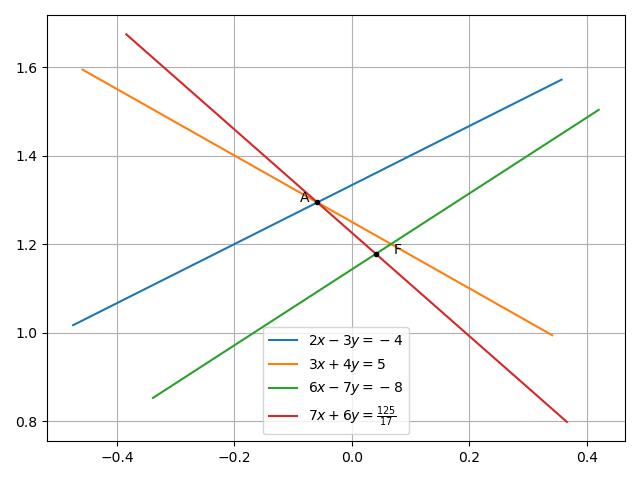
\includegraphics[width=\columnwidth]{chapters/11/10/4/24/figs/crossing.png}
        \caption{AF is the required line.}
        \label{fig:chapters/11/10/4/24/crossing}
    \end{figure}
	\item Find the equation of the line passing through the point of intersection of the lines $4x + 7y - 3 = 0$ and $2x - 3y + 1 = 0$ that has equal intercepts on the axes.\\
	\solution 
	  %Given lines can be written in the form of \begin{align}
        \Vec{n}^{\top}\Vec{x} = c
    \end{align}
   Therefore,
		\begin{align}
       \myvec{4&7}\vec{x}=3
       \label{eq:11/10.4/12/2}
   \end{align} 
   \begin{align}
       \myvec{2&-3}\vec{x}=-1
       \label{eq:11/10.4/12/3}
   \end{align}
   Now, line equation that has equal intercepts on the axes is
   \begin{align}
       \myvec{1 & 1}\Vec{x}=c
       \label{eq:11/10.4/12/4}
   \end{align}
   Solving equations \eqref{eq:11/10.4/12/2} and \eqref{eq:11/10.4/12/3}
		augumented matrix is
 \begin{align}
    \myvec{4&7&3\\2&-3&-1}\\
    \xleftrightarrow{R_1 \leftarrow 4 R_1}
    \myvec{1&\frac{7}{4}&\frac{3}{4}\\2&-3&-1}
    \xleftrightarrow{R_2 \leftarrow R_2 - 2R_1}
    \myvec{1&\frac{7}{4}&\frac{3}{4}\\0&\frac{-13}{2}&\frac{-5}{2}}\\
    \xleftrightarrow{R_2 \leftarrow \frac{-2}{13}R_2}
    \myvec{1&\frac{7}{4}&\frac{3}{4}\\0&1&\frac{5}{13}}
    \xleftrightarrow{R_1 \leftarrow R_1-\frac{7}{4}R_2}
    \myvec{1&0&\frac{1}{13}\\0&1&\frac{5}{13}}
\end{align}
Therfore, \begin{align}    
\vec{x} = \myvec{\frac{1}{13}\\\frac{5}{13}}
\end{align}
Also this point lies on the equation \eqref{eq:11/10.4/12/4}
\begin{align}
    \myvec{1 & 1}\myvec{\frac{1}{13}\\\frac{5}{13}} = c\\
    \frac{1}{13}+\frac{5}{13} = c
    \end{align}
    Therefore, the equation is \begin{align}
        \myvec{1&1}\Vec{x}=\frac{6}{13}
    \end{align}

\begin{figure}[!htbp]
    \centering
    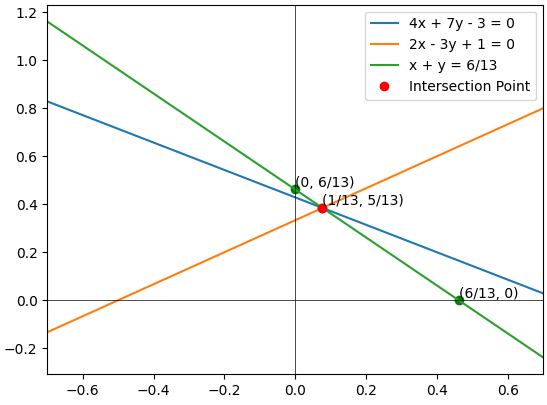
\includegraphics[width=\columnwidth]{chapters/11/10/4/12/figs/straightline.png}
    \caption{Straight Lines}
    \label{fig:enter-label}
\end{figure}
\item  Point $\vec{P}(0,2)$ is the point of intersection of $y$-axis and perpendicular bisector of line segment joining the points $\vec{A}(-1,1) \text{ and } \vec{B}(3,3)$
\item Prove that in any $\triangle{ABC}$, cos A=$\frac{b^2+c^2-a^2}{2bc}$, where a,b,c are the magnitudes of the sides opposite to the vertices A,B,C respectively.
\item The vector having intial and terminal points as (2,5,0)and (-3,7,4),respectively is
	\begin{enumerate}
\item -$\hat{i}+12\hat{j}+4\hat{k}$
\item $5\hat{i}+2\hat{j}-4\hat{k}$
\item $5\hat{i}+2\hat{j}+4\hat{k}$
\item $\hat{i}+\hat{j}+\hat{k}$
\end{enumerate}
\item The value of $\lambda$ for which the vectors $3\hat{i}-6\hat{j}+\hat{k}$ $\text{and}$,  $2\hat{i}-4\hat{j}$+$\lambda\hat{k}$ are parallel is
	\begin{enumerate}
\item $\frac{2}{3}$
\item $\frac{3}{2}$
\item $\frac{5}{2}$
\item $\frac{2}{5}$
	\end{enumerate}	
\item The value of the expression $\abs{\vec{a}\times\vec{b}}$+ $({\vec{a}.\vec{b}})$ is \rule{1cm}{0.15mm}.
\item If $\abs{\vec{a}\times\vec{b}}^2$ + $\abs{\vec{a}.\vec{b}}^2$=144 $\text{and}$  $\abs{\vec{a}}$=4, then $\abs{\vec{b}}$ is equal to \rule{1cm}{0.15mm}.
\item  Find the position vector of a point A in space such that $\overrightarrow{OA}$ is inclined at 60 $\degree$ to OX and at 45 $\degree$ to OY and $\abs{\overrightarrow{OA}} =10$ units.
\item Distance of the point $(\alpha \beta \gamma)$ from y-axis is
\begin{enumerate}
	\item $\beta$ 
	\item $\abs{\beta}$
	\item $\abs{\beta+\gamma}$
	\item $\sqrt{\alpha^2+\gamma^2}$
\end{enumerate}
\item If the directions cosines of a line are $k,k,k,$ then
\begin{enumerate}
	\item $k>0$
	\item $0<k<1$
	\item $k=1$ 
	\item $k=\dfrac{1}{\sqrt{3}}$ or $-\dfrac{1}{\sqrt{3}}$
\end{enumerate}
\item The reflection of the point $(\alpha \beta \gamma )$ in the xy-plane is 
\begin{enumerate}
	\item $\alpha,\beta,0)$
	\item $(0,0,\gamma)$
	\item $(-\alpha,-\beta,\gamma)$
	\item $(\alpha,\beta,-\gamma)$
\end{enumerate}
\end{enumerate}
